\section{Background and Problem}
\label{sec:background}

In this section, we provide background on dimensionality reduction (DR) and our problem of workload-aware DR.

\subsection{Dimensionality Reduction}
\label{sec:defs}

The goal of DR is to find a low-dimensional representation of a dataset that preserves properties of interest, such as data point similarity~\cite{dr-survey1,dr-survey2}. Formally, consider a data matrix $X \in \mathbb{R}^{\mvar \times \dvar}$, where each row $i$ corresponds to data point $x_i \in \mathbb{R}^\dvar$, with $\mvar > \dvar$.  
DR computes a transformation function $T: \mathbb{R}^\dvar \rightarrow \mathbb{R}^k$ that maps each $x_i$ to a more compact representation, resulting in a new data matrix $T(X) = \tilde{X} \in \mathbb{R}^{\mvar \times k}$.

\subsubsection*{Principal Component Analysis (PCA)}
\label{sec:pca}
PCA is a linear DR technique that identifies a new orthogonal basis for a dataset that captures its directions of highest variance.
Of all linear transformations, this basis minimizes reconstruction error in a mean square sense. 
Classically implemented PCA uses a Singular Value Decomposition (SVD) routine~\cite{trefethen}.


\begin{comment} 
\begin{algorithm}
\begin{algorithmic}[1]
\Statex \textbf{Inputs:}  
\Statex $X \in \mathbb{R}^{m_1 \times d}$: training data matrix 
\Statex $Y \in \mathbb{R}^{m_2 \times d}$: data matrix to transform 
\Statex $k \in \mathbb{Z}_+$: desired dimensionality of transformed data
\Statex \textsc{SVD-T}: any truncated SVD algorithm  
\Statex
\Statex \hrule
\Function{fit}{$X$}:
	\State $\bar{X} = \text{columnMeans}(X)$
	\State $C_X = X - \bar{X}$
		\Comment{$C_X \in \mathbb{R}^{m_1 \times d}$}
	\State \textbf{Store: } $\bar{X}, C_A$
\EndFunction

\Function{transform}{$Y, k, $ \textsc{SVD-T}}:
	\State $U, \Sigma, V^T$ = \textsc{SVD-T}$(C_X, k)$
		\Comment{$V \in \mathbb{R}^{d \times k}$}
	\State $C_Y = Y - \bar{X}$
		\Comment{$C_Y \in \mathbb{R}^{m_2 \times d}$} 
	\State \textbf{Store: } $T = V$ 
			\Comment{Cache for repeated use} \\
	\Return $C_YT$
		%\Comment{$C_BV \in \mathbb{R}^{M_2 \times k}$} 
\EndFunction

\end{algorithmic}
\caption{PCA via truncated SVD}
\label{alg:PCA-inc}
\end{algorithm}

%discuss advanced techniques
As described in \S\ref{related}, several theoretical advances provide accelerated means of of efficiently computing PCA over large-scale data beyond the na\"ive SVD-based approach.
These methods operate on samples of input data, and---in theory---confer substantial runtime benefits when in fact a low-dimensional basis exists (i.e., the spectrum of eigenvalues has a large drop).
However, there are two main challenges in utilizing these approaches.
First, it is unclear when to stop sampling data points when using stochastic or mini-batch methods, including state-of-the-art momentum techniques that achieve accelerated convergence rates~\cite{CDS}.
This is because convergence of these techniques (e.g., the magnitude of the gradient in stochastic gradient methods) does not correspond directly to preservation of metrics of interest.
Second, these techniques typically rely the target reduced dimension ($k$) to be specified a priori, but the suitable $k$ for the task at hand is rarely known a priori for a given dataset. The choice of $k$ can dramatically affect runtimes and convergence rates, making the target dimensionality an important, yet difficult to obtain parameter. 

Thus, even with advanced techniques, it is unclear \emph{how much computation is required} to obtain acceptable low dimensional representations, and \emph{how low a dimension is considered acceptable} for specific application constraints. 
We describe how DROP overcomes these challenges in [forward ref sampling], and show how answering these questions enables improvements over previous techniques when evaluated in an end-to-end context.  
\end{comment}

\subsection{DR \red{for Repeated-Query Workloads}}

In workloads such as similarity search, clustering, \red{or classification}, ML models are periodically trained over historical data, and are \emph{repeatedly queried} as incoming data arrives or new query needs arise. 
Indexes built over this data can improve the efficiency of this repeated query workload in exchange for a preprocessing overhead.
DR with a multidimensional index structure in the reduced space is a classic way of achieving this~\cite{local-dr,dynamic-ss,dm-book,humming-index,decade,search}.
% a metric-preserving transformation reduces input dimensionality, and an index is built in this new space for subsequent queries.


\subsubsection*{\red{DR in Similarity Search}}
Similarity search is a repeated-query workload performed over data types including images, documents and time series~\cite{keogh-study,lsh}.
In the common setting where similarity is measured by Euclidean distance, our goal is to find a low-dimensional representation that approximately preserves pairwise $\ell_2$-distances between data points. We quantify this distance-preservation property using the Tightness of Lower Bounds ($TLB$) metric~\cite{keogh-study}:  
%The Tightness of Lower Bounds ($TLB$) is typically the metric preserved by DR in this setting~\cite{keogh-study}, as it measures how well a \emph{contractive} transformation (i.e. distances in the transformed space are less than or equal to those in the original) preserves pairwise distances. 
%It can estimate the accuracy of a low dimensional transformation without performing the similarity search task:
\begin{equation}
\label{eq:tlb}
TLB = \frac{2}{\mvar(\mvar-1)}\sum_{i<j}\frac{\| \tilde{x}_i -  \tilde{x}_j \|_2 }{\| x_i -  x_j\|_2 }.
\end{equation}

Given the large amount of research in the space, we use time series similarity search as a running case study throughout this paper. 
We briefly revisit a comparison of DR techniques for time series similarity search from VLDB 2008~\cite{keogh-study} to verify that PCA can outperform conventionally used techniques (low $k$), but with a high DR runtime cost.
The authors omit PCA due to it being ``untenable for large data sets." 

We compare PCA via SVD to baseline techniques based on returned dimensionality and runtime with respect to $TLB$ over the largest datasets from~\cite{keogh-study}. 
We use their two fastest methods as our baselines as they show the remainder exhibited ``very little difference'': Fast Fourier Transform (FFT) and Piecewise Aggregate Approximation (PAA).
On average, PCA admits an output dimension $k$ that is $2.3\times$ (up to $3.9\times$) and $3.7\times$ (up to $26\times$) smaller than PAA and FFT for $TLB = 0.75$, and $2.9\times$ (up to $8.3\times$) and $1.8\times$ (up to $5.1\times$) smaller for $TLB = 0.99$.
However, PCA implemented via out-of-the-box SVD is on average over \red{$26\times$ (up to $56\times$)} slower than PAA and over \red{$4.6\times$ (up to $9.7\times$)} times slower than FFT when computing the smallest $TLB$-preserving basis.
While the margin between PCA and alternatives is dataset-dependent, PCA almost always preserves $TLB$ with a lower dimensional representation at a higher runtime cost.
This runtime-dimensionality tradeoff motivates our study of workload-aware DR methods. 

\begin{figure}
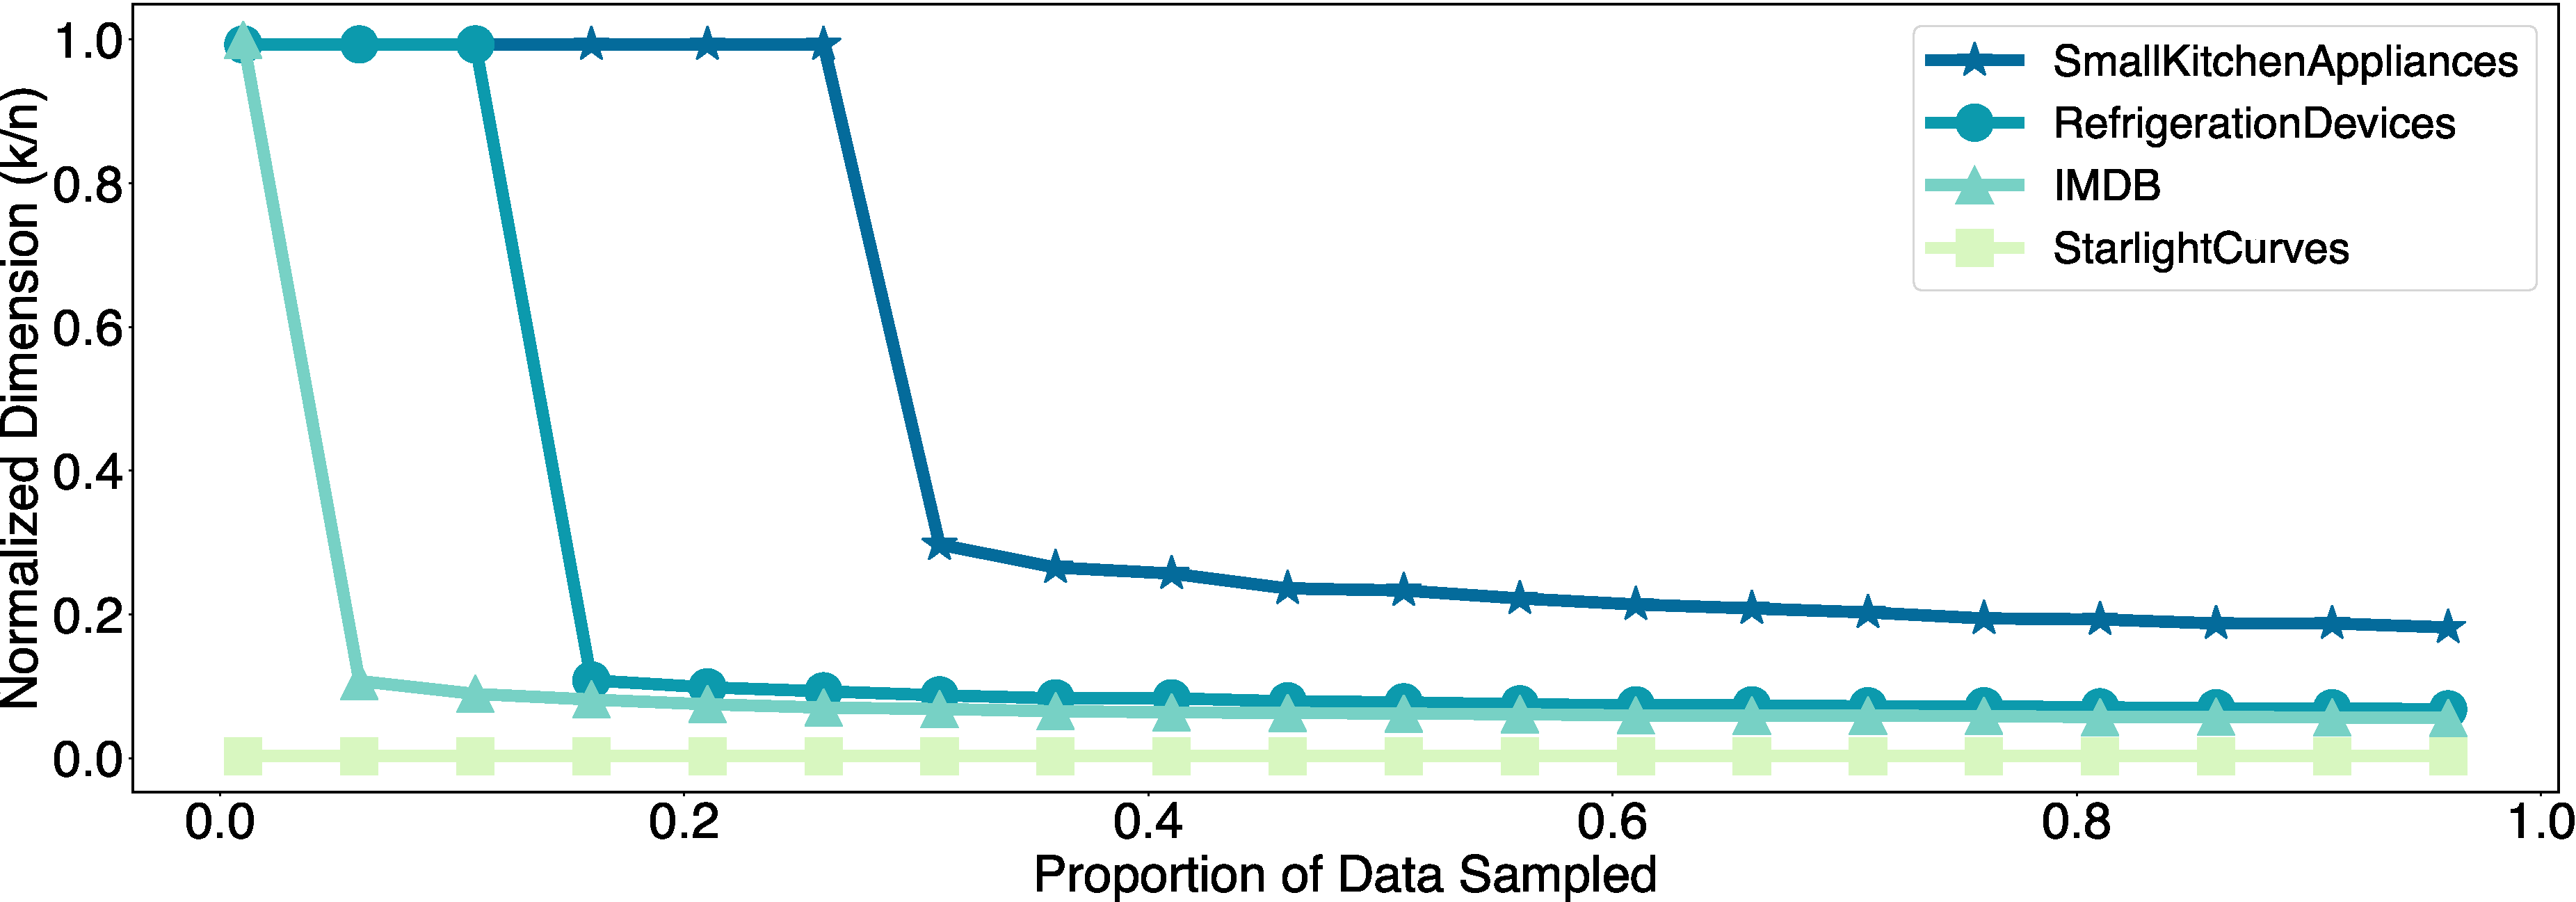
\includegraphics[width=\linewidth]{figs/progressive.pdf}
\caption[]{ Improvement in representation size for  $TLB = 0.80$ across three datasets. Higher sampling rates reduce dimension until reaching a state equivalent to running PCA over the full dataset ("convergence").}
\label{fig:progressive}
\end{figure}


\subsection{Problem: Workload-Aware DR}
\label{subsec:wadr}

In workload-aware DR, we perform DR to minimize workload runtime subject to downstream metric constraints.
DR is a fixed cost (i.e., index construction for similarity search), while workload queries incur a marginal cost dependent on DR dimensionality (i.e., nearest neighbor query). 

As input, consider a dataset $X$, target metric preservation $B$ (e.g., $TLB \geq .99$), and optional downstream runtime model as a function of dimensionality $\mathcal{C}_\mvar(\dvar)$ for an $\mvar\times \dvar$ matrix.  
Denoting DR runtime as $R$, we define the problem:
\begin{problem}
\label{def:opt}
  Given $X \in \mathbb{R}^{\mvar \times \dvar}$, $TLB$ constraint $B \in 
  (0, 1]$, confidence $c$, and workload runtime function $\mathcal{C}_\mvar:\mathbb{Z}_{+} \rightarrow \mathbb{R}_{+}$, find $k$ and transformation
  matrix $T_k \in \mathbb{R}^{\dvar \times k}$ that minimizes $R + \mathcal{C}_\mvar(k)$
  such that $TLB(XT_k) \geq B$ with confidence $c$.
\end{problem}

We assume $\mathcal{C}_\mvar(\dvar)$ is monotonically increasing in $\dvar$.
%as the premise of DR for efficient analytics relies on downstream tasks running faster on lower dimensional data.
%Absent the cost model, we default to execution until convergence (i.e, until $k$ plateaus) as described in \S\ref{sec:sampling}, and demonstrate the cost of doing so in \S\ref{sec:experiments}.
The more DR time spent, the smaller the transformation (as in the case study), thus the lower the workload runtime.
To minimize $R + \mathcal{C}_\mvar(k)$, we  determine how much time to spend on DR (thus, what $k$ to return) to minimize overall runtime.

\begin{figure*}
\begin{center}
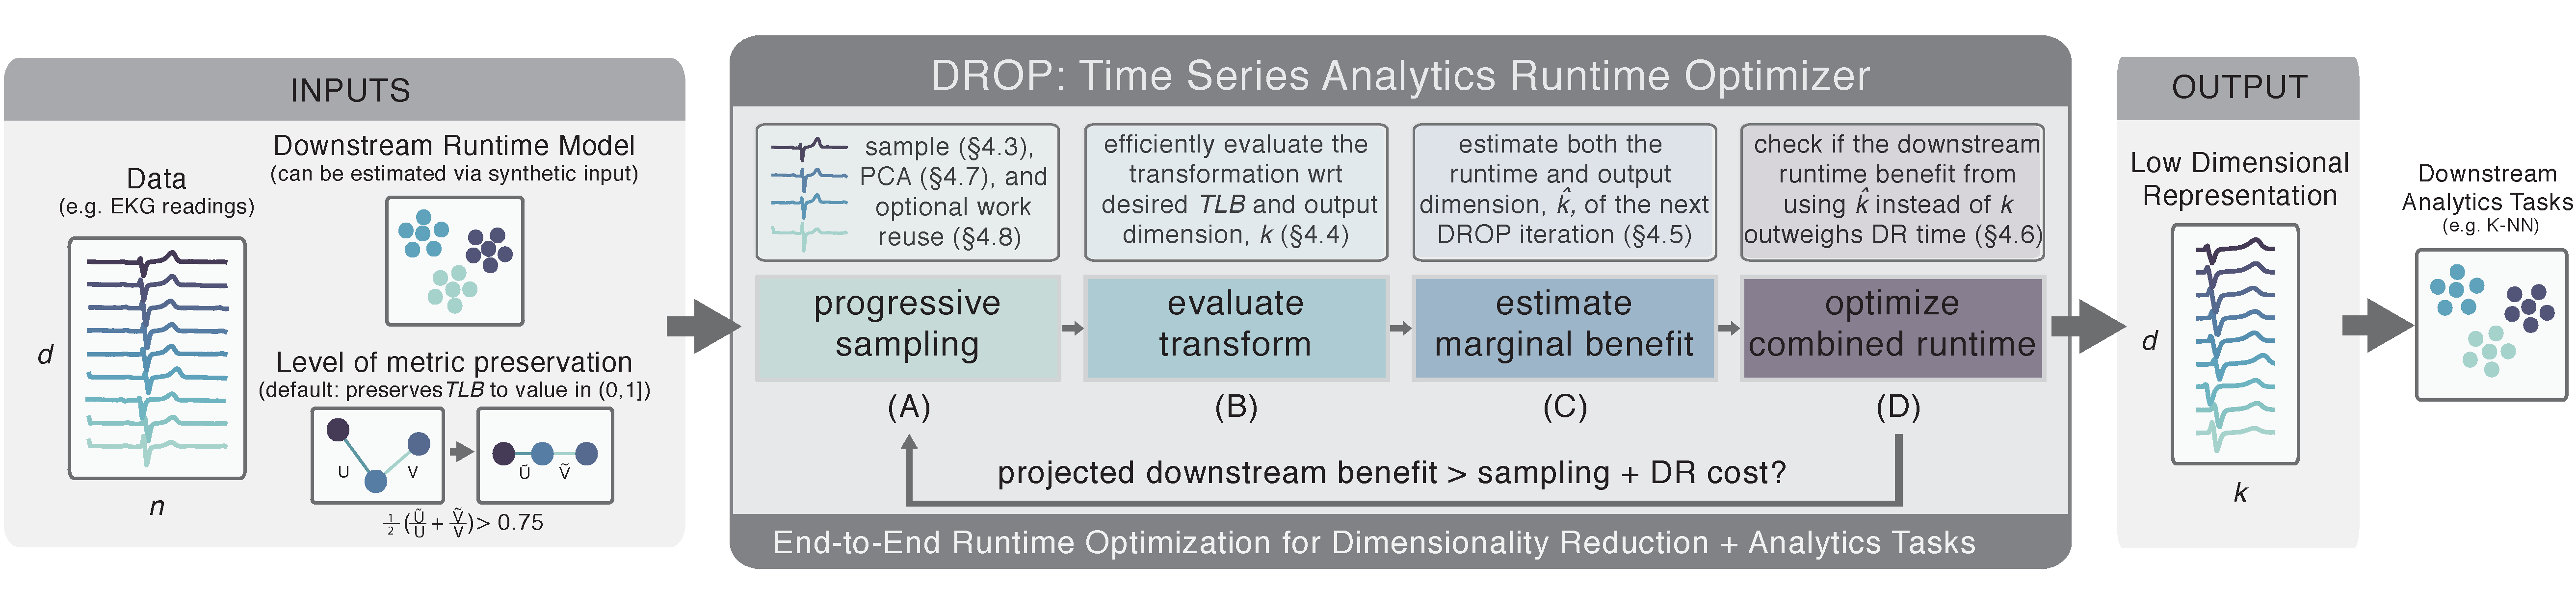
\includegraphics[width=\textwidth]{figs/system_arch.pdf}\vspace{-1em}
\caption[]{High-level DROP architecture depicting DROP's inputs, outputs, and core components.}
\end{center}
\vspace{-1em}
\label{fig:arch}
\end{figure*}


\subsection{Solution Sketch: Progressive Sampling}
\label{sec:sampling}


Inspired by stochastic PCA methods (\S\ref{sec:relatedwork}), we turn to sampling to tackle workload-aware DR. 
Many real-world \red{datasets} are intrinsically low-dimensional, as evidenced by their rapid falloff in their eigenvalues, so running PCA over data samples generalizes well. 
To verify, we extend our case study by varying the target $TLB$ and examining the minimum number of uniformly selected samples required to obtain a $TLB$-preserving transform with $k$ equal to input dimension $\dvar$.
On average, a sample of under $0.64\%$ $(\text{up to } 5.5\%)$ of the input is sufficient for $TLB = 0.75$, and under $4.2\%$ $(\text{up to } 38.6\%)$ is sufficient for $TLB=0.99$.  
If this sample rate is known, we obtain up to \red{$91\times$ speedup} over PCA via SVD.%---with no algorithmic improvement. 

However, this benefit is dataset-dependent, and unknown a priori.
We thus turn to progressive sampling (gradually increasing the sample size) to identify how large a sample suffices.
Figure~\ref{fig:progressive} shows how the dimensionality required to attain a given $TLB$ changes when we vary dataset and proportion of data sampled.
Increasing the number of samples (which increases PCA runtime) provides lower $k$ for the same $TLB$.
However, this decrease in dimension plateaus as the number of samples increases.
Thus, while progressive sampling would allow us to tune the amount of time spent on DR, we must determine when the downstream value of decreased dimension is overpowered by the cost of DR---that is, whether to sample to convergence or terminate early (e.g., at $0.3$ proportion of data sampled for SmallKitchenAppliances). 






